\documentclass{article}
\usepackage{tikz, comment}
\usepackage{pifont}
\usepackage{fontspec}
\usetikzlibrary{arrows, decorations.markings, decorations.pathreplacing}
\begin{comment}
:Title: Not defined yet
:Tags: area using polar coordinates, polar integral formula ;sohcahtoa;sine, sin ;polar form of a complex number;cis
:Prob: 0.4128;0.4095;0.4066;0.4058;0.375
:Slug: No name yet

Description Here.........
\end{comment}
\begin{document}\centering

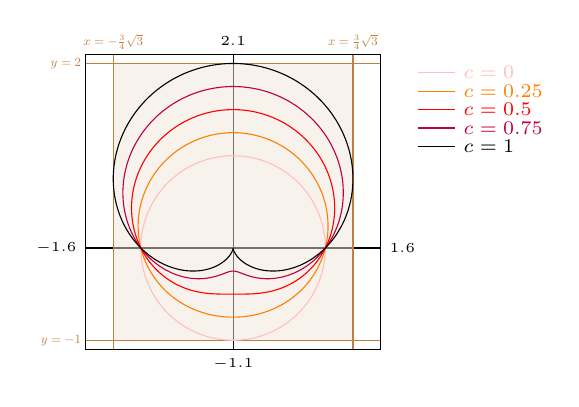
\begin{tikzpicture}[>=latex,xscale=0.375*10/3.2, yscale=0.375*10/3.2][font=\sf\small]

%\draw[xstep=1cm,ystep=1cm,color=gray!20] (-2, -2) grid (2, 2);

\draw[] (-1.6, 0) -- (1.6, 0);
\draw[] (0, -1.1) -- (0, 2.1);

\node[left] at (-1.6, 0) {\tiny$-1.6$};
\node[right] at (1.6, 0) {\tiny$1.6$};
\node[below] at (0, -1.1) {\tiny$-1.1$};
\node[above] at (0, 2.1) {\tiny$2.1$};

\draw [pink] (1.6+0.4, {2.1-1*0.2}) --++(0.4, 0)node[right] {\scriptsize$c=0$};
\draw [orange] (1.6 +0.4, {2.1-2*0.2}) --++(0.4, 0)node[right] {\scriptsize$c=0.25$};
\draw [red] (1.6 +0.4, {2.1-3*0.2}) --++(0.4, 0)node[right] {\scriptsize$c=0.5$};
\draw [purple] (1.6 +0.4, {2.1-4*0.2}) --++(0.4, 0)node[right] {\scriptsize$c=0.75$};
\draw [black] (1.6 +0.4, {2.1-5*0.2}) --++(0.4, 0)node[right] {\scriptsize$c=1$};

\draw[brown, samples=100, smooth, domain=1.6:-1.6, variable=\x]
plot ({\x}, {2}) node[left, scale=0.5] {$y=2$}; %y=2

\draw[brown, samples=100, smooth, domain=1.6:-1.6, variable=\x]
plot ({\x}, {-1}) node[left, scale=0.5] {$y=-1$}; %y=-1

\draw[brown, samples=100, smooth, domain=-1.1:2.1, variable=\y]
plot ({3/4*sqrt(3)}, {\y}) node[above, scale=0.5] {$x=\frac{3}{4}\sqrt 3$}; %y=-1

\draw[brown, samples=100, smooth, domain=-1.1:2.1, variable=\y]
plot ({-3/4*sqrt(3)}, {\y}) node[above, scale=0.5] {$x=-\frac{3}{4}\sqrt 3$}; %y=-1

\clip[draw] (-1.6, -1.1) rectangle (1.6, 2.1);

\draw[brown, fill opacity=0.5, fill=brown!20]
plot ({-3/4*sqrt(3)},{-1})--({3/4*sqrt(3)},{-1})--({3/4*sqrt(3)},{2})--({-3/4*sqrt(3)},{2})--cycle;

\draw[pink, samples=100, smooth, domain=0:2*pi, variable=\t]
plot ({(1+(0)*sin(\t r))*cos(\t r)}, {(1+(0)*sin(\t r))*sin(\t r)}); %c=0

\draw[orange, samples=100, smooth, domain=0:2*pi, variable=\t]
plot ({(1+(0.25)*sin(\t r))*cos(\t r)}, {(1+(0.25)*sin(\t r))*sin(\t r)}); %c=0.25

\draw[red, samples=100, smooth, domain=0:2*pi, variable=\t]
plot ({(1+(0.5)*sin(\t r))*cos(\t r)}, {(1+(0.5)*sin(\t r))*sin(\t r)}); %c=0.5

\draw[purple, samples=100, smooth, domain=0:2*pi, variable=\t]
plot ({(1+(0.75)*sin(\t r))*cos(\t r)}, {(1+(0.75)*sin(\t r))*sin(\t r)}); %c=0.75

\draw[black, samples=100, smooth, domain=0:2*pi, variable=\t]
plot ({(1+(1)*sin(\t r))*cos(\t r)}, {(1+(1)*sin(\t r))*sin(\t r)}); %c=1

\end{tikzpicture}
\end{document}